\documentclass{article}
\usepackage[colorlinks]{hyperref}% hyperlinks [must be loaded after dropping]
\hypersetup{colorlinks,breaklinks,
citecolor = blue,
urlcolor=blue,
linkcolor=blue}
\usepackage{graphicx}
\usepackage{subfig}
\usepackage{float}
\usepackage{enumitem,amssymb}
\usepackage[margin=0.5in]{geometry}
\usepackage[capitalise]{cleveref}
\usepackage{listings}
\lstset{
basicstyle=\small\ttfamily,
columns=flexible,
breaklines=true
}

\newlist{todolist}{itemize}{2}
\setlist[todolist]{label=$\square$}
\setlength\parindent{0pt}

\begin{document}

\begin{center}
\begin{LARGE}
\textbf{Matlab to C++ ``Automatic" Translation \\ Journey \& Lessons Learned }\\
\end{LARGE}
\vspace{8pt}
%Internal Use Only
\end{center}

\section{Preface}

Matlab has been and will continue to be utilized for many scientific computing roles.  At some point in a project's lifetime however, the personnel using a Matlab code may need to move to a different platform for one reason or another (ease of public release, performance issues, supercomputing capability, excessive cost, etc...).  While Matlab has created a way to automatically translate Matlab code into C or C++, it has some gotchas.  I advise the reader review this lessons learned document to determine the best route for their project.  

\section{Simple C++ Automatic Translation}
I followed this \href{https://www.mathworks.com/videos/automatically-converting-matlab-code-to-c-code-96483.html}{tutorial} for a several line example and compiled the output on the skybridge linux cluster using:
\begin{verbatim}
cc main.cpp test_function.cpp test_function_terminate.cpp -o pleasework
\end{verbatim}

%Skybridge can be accessed on a terminal/prompt with SSH, and small files can be transferred with sftp (both if on the SRN directly or via VPN).
%\begin{verbatim}
%ssh username@skybridge
%sftp username@skybridge
%\end{verbatim}

This simple example was quite easy, straightforward, and the C++ output code was relatively organized and understandable.  Encouraging, but what about the other option for spinning up a code into a distributable program?

\subsection{Application Compiler}
Now switching to the application compiler: I had issues trying to get it to create an installer with the runtime included. (I.e. this option does not need a Matlab license, but it does run the Matlab runtime in the background, which is a fairly large level of overhead.) I installed the Matlab runtime from NILE, but after a half hour of trying to get it to connect up with my instance of Matlab in the Application Compiler, I stopped. I'm sure it can be done, it just isn't obvious. The web installer works just fine and does output prebuilt executables as well, which run, but there is a lot of overhead time for it to start. My simple function (from the tutorial above) just output a few things to the terminal, so I couldn't just double click the executable since it wouldn't show anything, I ran it from the terminal (using a mac) to see the output.

\begin{verbatim}
cd directory/that/binary/is/located
./binary
\end{verbatim}

This may be an option for relatively simple programs where performance isn't really and issue and you/the customer doesn't mind having to wrestle with the Matlab runtime.  Let's switch back to the automatic translator, but this time with a more complex code.

\section{Automatic Translation of a More Complex Matlab Code}

So, the simple case seemed to work great, and the output C++ code was understandable.  However, we now switch to the laborious process required for a complex code.  I used a 12,000 line code for the characterization of vertical axis wind turbine structural dynamics (OWENS).  I went through the process of 1) addressing the debugger suggestions, 2) addressing the code readiness suggestions (right click on file in Matlab GUI (graphical user interface (\cref{fig:code_readiness_both}) to select code readiness), 3) addressing the Matlab coder errors (via the Matlab coder app accessed from within the GUI \cref{fig:coder_beginning}), and 4) addressing compiling/runtime errors \cref{fig:coder_end}.  The coder list of errors was sometimes misleading since many of the problems it listed stemmed from another problem.  By focusing on just the issue at the top of the stack and rerunning each time, I was able to get through them all (though not until after nearly 100 commits).  There were something like 300 issues the first three items, then a hundred more or so in the last, with the distribution of effort falling approximately in the following way:

\begin{itemize}

  \item 10\% Matlab editor suggestions
	  \subitem - Simple syntax/declaration suggestions
  \item 70\% Matlab code readiness and coder GUI
	  \subitem - Replacing Unsupported Built in Functions
	  \subitem - Variable Type Declaration
	  \subitem - Variable Size Declaration
	  \subitem - Explicate Indexing
	  \subitem - Variable Scope on All Execution Paths
  \item 20\% Matlab Auto Generated MEX Test Function - Runtime Errors
	  \subitem - Variable type/size/indexing/scope issues not caught by coder

\end{itemize}

I created a set of unit tests and ran them after each set of changes in the code to isolate when I made breaking changes. I also used git to track the changes, enabling me to easily revert to a prior state when I found a particular method of changes was not going to work out in the end. \\

In summary, the coder requires the user to rewrite the code with a restricted set of tools in a hierarchy as if it was a typed language; all variables must be declared before use or initialized in such a way that the variable type is known (like the output of a function where the internal types being passed up are known), and the variable type and size must be consistent over all execution paths.  Many of the methods required to satisfy these requirements in the base Matlab language were non-intuitive, but will be spelled out in this document.  All in all, I'd say this part was about half as intensive as if I were to just have ported over to a different language.

\begin{figure}[htbp!]
    \centering
        \subfloat[Code readiness utility and MATLAB Coder app locations.]{
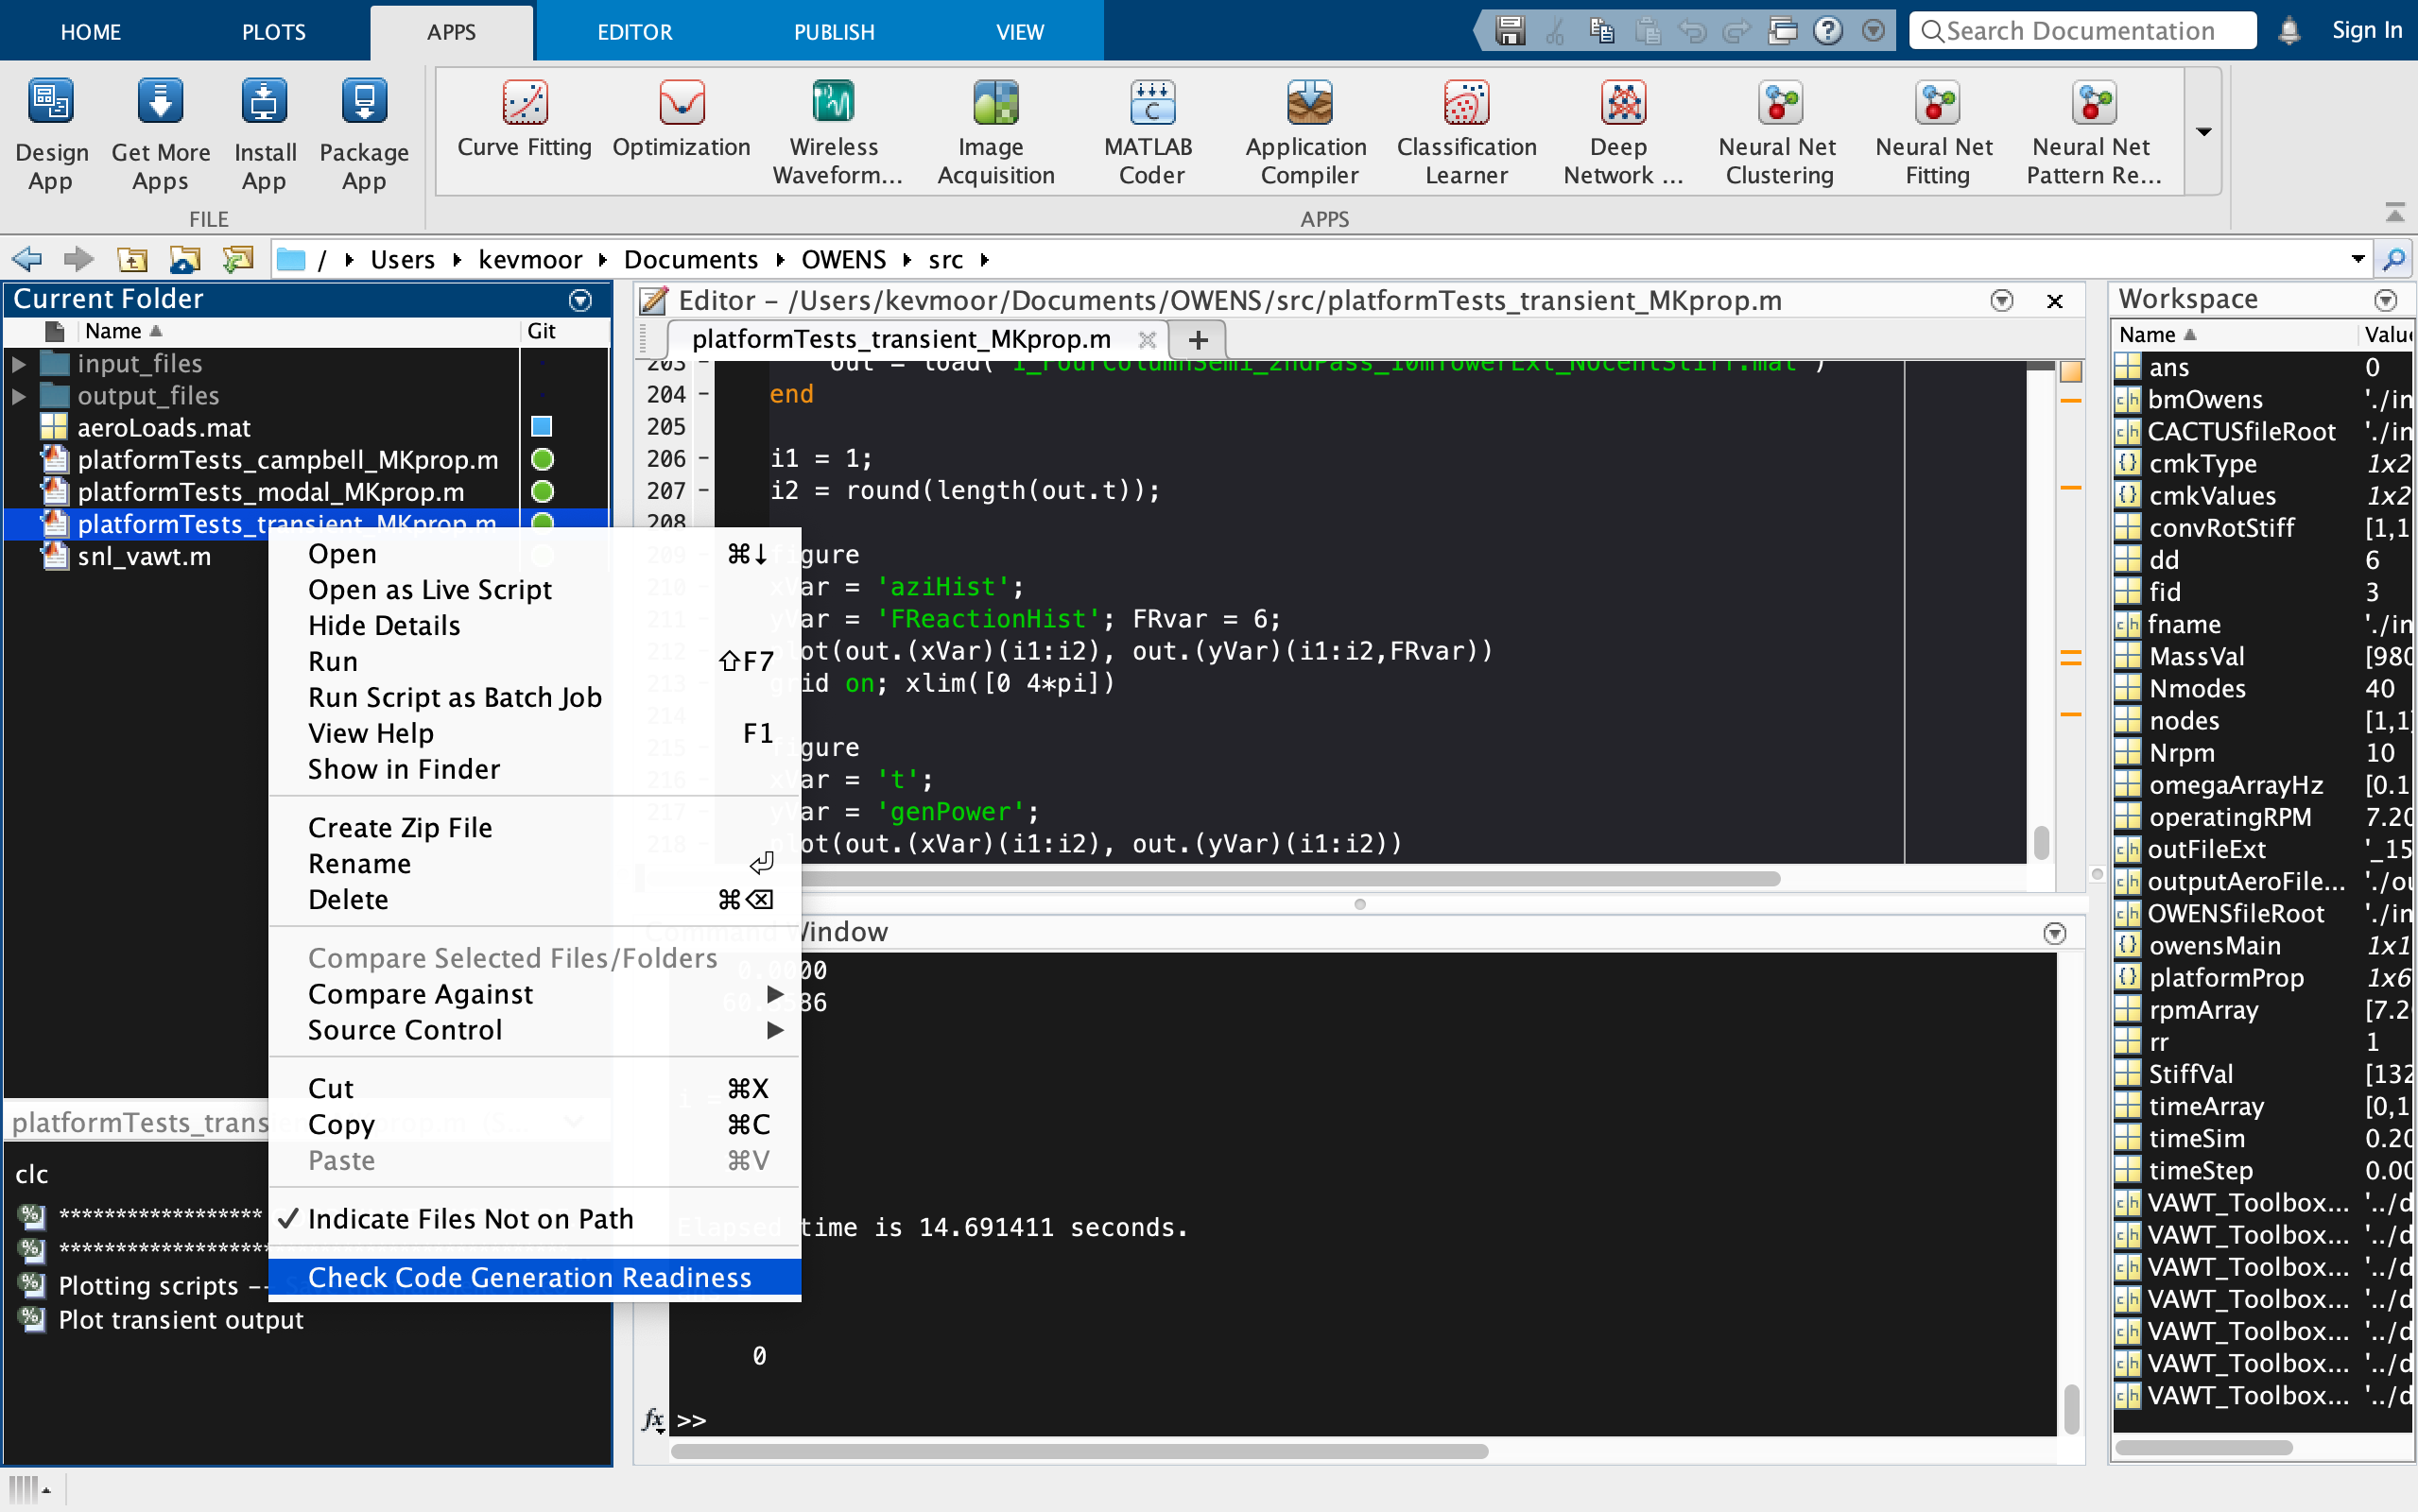
\includegraphics[trim={2cm 0cm 20cm 0},clip,width=0.40\textwidth]{../figs/CodeReadiness.png}

\label{fig:CodeReadiness}
    }
    \qquad
    \subfloat[Transient Vertical force.]{
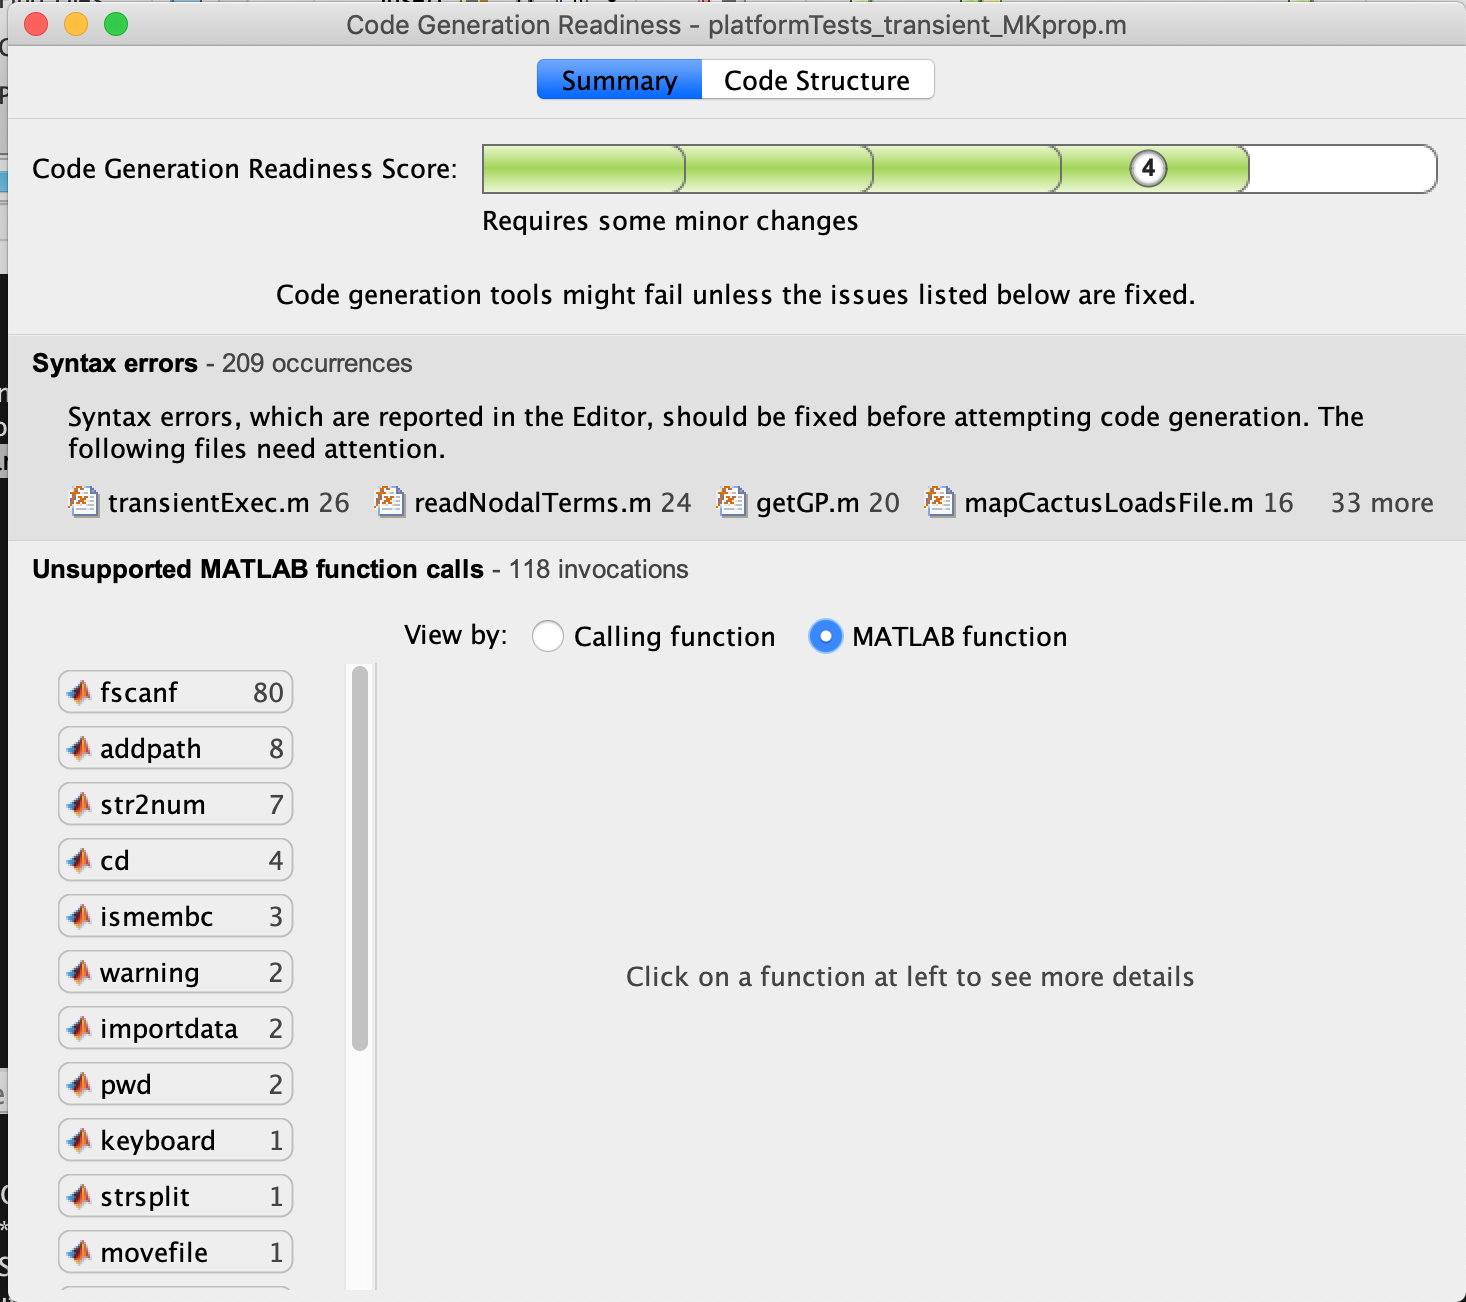
\includegraphics[trim={.4cm 0cm 1cm 0},clip,width=.52\textwidth]{../figs/readiness_output_start.png}
    \label{fig:readiness_output_start.png}
    }
    \caption{Code readiness utility output at beginning of process showing about 300 issues}
    \label{fig:code_readiness_both}
\end{figure}



\begin{figure}[H]
\centering
%\vspace{-12pt}
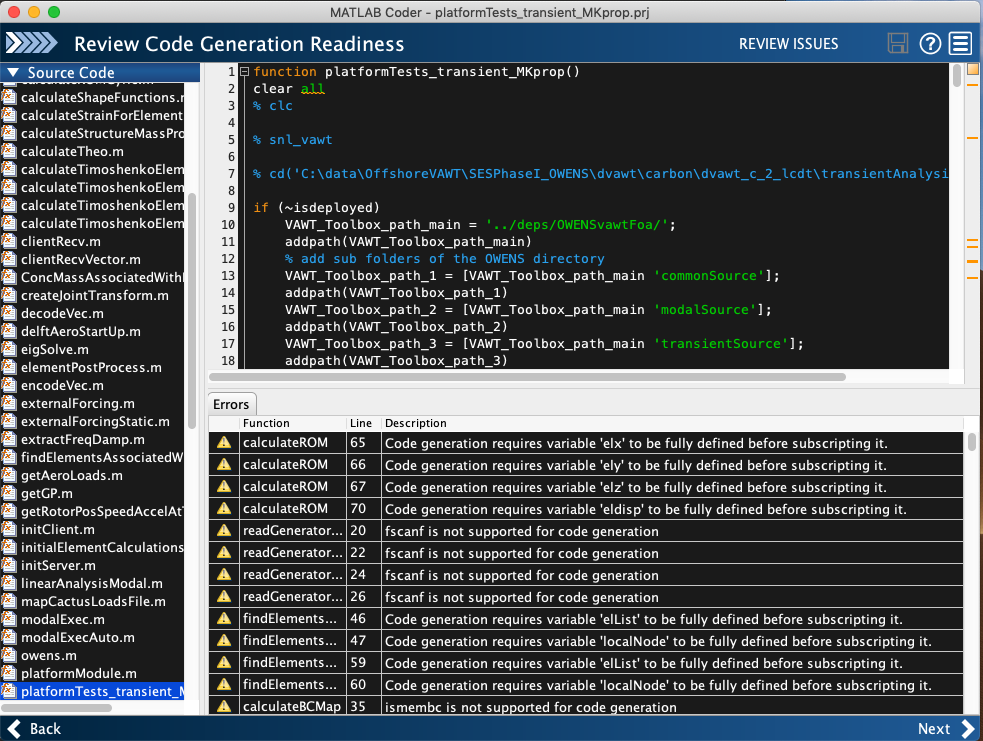
\includegraphics[trim={0 0 0cm 0},clip,width=0.9\textwidth]{../figs/coder_beginning.png}
%\vspace{-12pt}
\caption{Coder output at beginning.}
\label{fig:coder_beginning}
\end{figure}

\begin{figure}[H]
\centering
%\vspace{-12pt}
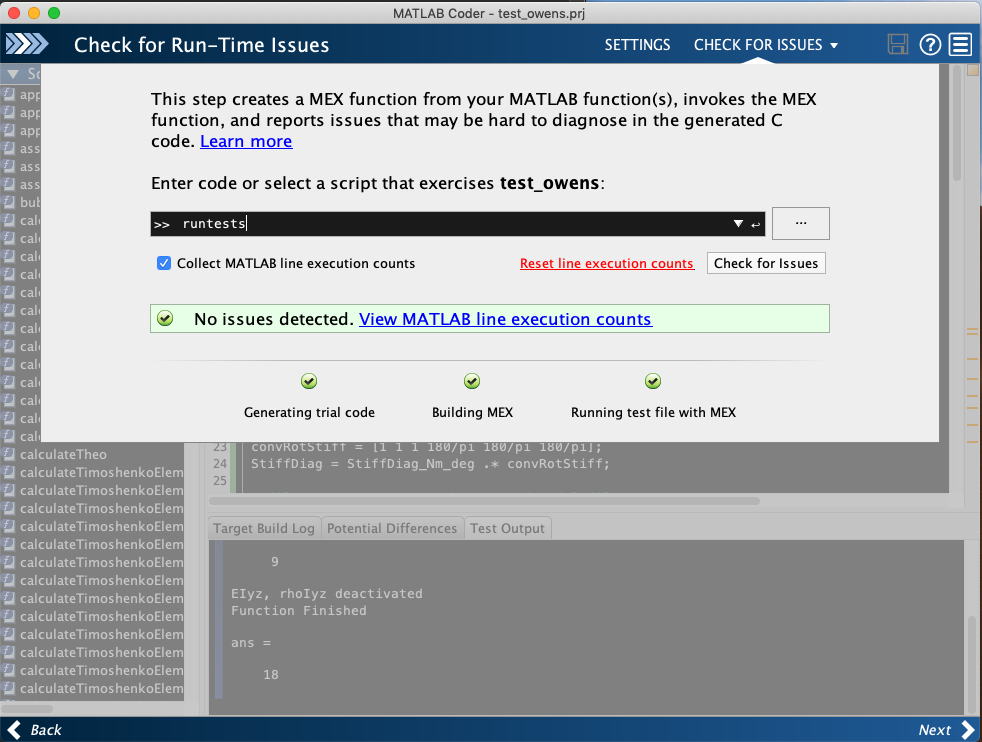
\includegraphics[trim={0 0 0 0},clip,width=0.7\textwidth]{../figs/coder_end.png}
%\vspace{-12pt}
\caption{Coder output with no errors left and Matlab auto generated mex test function successfully ran.}
\label{fig:coder_end}
\end{figure}

\subsection{Unsupported Functions and Resolutions}
The following \href{https://www.mathworks.com/help/simulink/ug/functions-and-objects-supported-for-cc-code-generation.html}{link} gives a list of the functions across the toolboxes that are supported.  The following is the list of unsupported functions per the code readiness tool and the solutions used:

\begin{itemize}

\item Fscanf - several other options in the list of supported functions, like fseek
\item Addpath - directly call out all paths, keep them in structures to be clean.
\item Str2num - use str2double
\item Cd - restructure code, see: \href{https://www.mathworks.com/help/compiler_sdk/ml_code/writing-deployable-matlab-code.html}{here}
\subitem - Robust way of extracting the file directory regardless of slash type
\begin{verbatim}
last_delimiter   = find(or(inputfile == '/', inputfile == '\'));
fdirectory       = inputfile(1:last_delimiter(end));
 \end{verbatim}
\item Ismembc - use ismember
\item Warning - convert to print statement
\item Importdata - use an approved file reading method from link, may have to write small function to get the right format
\item Pwd - same as cd
\item Keyboard - restructure code: should not be hitting the keyboard in the middle of a batch parallel run on a HPC cluster
\item Strsplit - write own splitter logic, or use something like strfind in the approved list
\item Movefile - restructure so moving is not needed, or read in and rewrite the file elsewhere, and then delete the original file.
\item Getframe - This has to do with creating a video. It is possible to restructure the code to simply output non-displayed saved images and post process them into a video. Also may be problematic to include image creation that uses gpu if there is no gpu on the cluster being run on, so may need to push to post processing, depends on if gpu is used etc.
\item Genpath - same as cd
\item VideoWriter - same as getframe
\item Textscan - same as fscanf
\item Movegui - same as getframe
\item Sscanf - same as fscanf
\item Clc - remove as it is matlab specific to the console. Could put in printing levels.
\item Unix - remove since this is specific to wavec, seems to be dependent on hard coded file paths, and could easily be unified for the coupling with the new hydro tool.
\item Eigs - use one of the other eigenvalue/vector functions from the link
\item Writetable - use something like fwrite or fprintf
\item Cell2mat - restructure to not require this type of conversion
\item Annotation - move to post processing or include in legend, or remove.

\end{itemize}

\subsection{Variable Declarations}

How to preinitialize arrays of structs:
\href{https://www.mathworks.com/help/simulink/ug/defining-arrays-of-structures-for-code-generation.html}{initialize structs}

Some best  \href{https://www.mathworks.com/help/simulink/ug/best-practices-for-defining-variables-for-c-c-code-generation.html}{practices}

\begin{itemize}

\item If the type is unchanging and easily inferred (i.e. not a for loop), then you don't have to declare it.
\item All variables used must be declared on all execution paths (i.e. must always have an else for each if, or be declared outside the if)
\item All if statements must have an else, or the equivalent such that all LOCAL execution paths possible are covered
\item Structs must be built in the same order on all execution paths and cannot be used until they are finished being constructed

\end{itemize}

\subsection{Side Notes}

As a side note, if you are interested in determining the subset of files called by a particular portion of code you are trying to translate: \href{https://www.mathworks.com/help/matlab/matlab_prog/identify-dependencies.html}{determine dependencies}\\

Also, to compile the code (since it had 100 separate c++ files, many of them being Matlab built in functions), I pulled in the example main.cpp and main.h files the coder generates in its output folder and compiled on the terminal via: (run from within the folder all the files are located)

\begin{verbatim}
c++ -std=c++11 -o3 *.cpp -o success_split
\end{verbatim}

I tried both C and C++ and they ran in about the same time, however letting Matlab handle the compiling is much faster as will be discussed later on.\\

%\vspace{12pt}

\section{Performance Considerations}

For all of this work (about 80 hours worth), we got a 3x \textbf{slowdown} right off the bat.  Not to mention the code has nearly 3x as many lines, and when you look at the code, it is not something that I'd want to mess with.  Sometimes Matlab simplifies the code, for example, if you say a=1, then c=a+2, it swaps out a for 1, directly in the code.  So, if you have portions commented out that use variables previously declared, the output code between the commended and uncommented versions can be drastically different. (Or if you are trying to include hooks for intended post-translation changes/coupling, it could get interesting.)  It also will expand certain operations directly on the spot, like matrix multiplication, leaving this incomprehensible large section where there should just be a function call and a separate function.  If you try to write that architecture in the first place (trying to put that example matrix multiply in a separate function), Matlab does not necessarily respect your structure and may just slap the messy 100 lines of code where your intended clean 1-liner function call should have been.  So, out of the box, the computational performance leaves much to be desired (though it does get better with some tweaks that will be discussed), and the output code makes the developer's ability to perform much more difficult.


\begin{center}
\begin{tabular}{|c| c c c c|}
 \hline
& Matlab & Matlab MEX & Compiled C++ & Octave \\
 \hline
Lines of Code & 12,110 lines  & NA & 29,375 lines & Runs .m file \\
\hline
Short (0.1s) and File Output & 21s & 34s & 61s & about 400s \\
\hline
Short (0.1s), No File Output & 14s & 19s & 60s & about 400s \\
\hline
LONG (19.1s), No File Output & 13m 40s (9s/100 ts) & 4m 31s (3s/100 ts) & 3hr (2min/100 ts) & 15hr (10min/100 ts) \\
\hline
\end{tabular}
\end{center}

\subsection{Profiling the Super Slow C++ Code}

I'm on a mac, so I was able to get the C++ debugger setup using homebrew on the terminal:

\begin{verbatim}
brew install gperftools
brew install graphviz
brew install ghostscript
\end{verbatim}


I had to disable address space layout randomization (ASLR) on the mac to get the debugger to work \href{https://stackoverflow.com/questions/10562280/line-number-in-google-perftools-cpu-profiler-on-macosx}{more info here}.  So in the end I ran the following commands to get the nice visual below. (Note that I had to change the default .svg program in finder.  I changed mine to safari)\\

\begin{verbatim}
    c++ -std=c++11 -lprofiler -g -Wl,-no_pie *.cpp -o please4work
    env CPUPROFILE=/tmp/prof.out ./please4work
    pprof --web --functions ./please4work /tmp/prof.out
\end{verbatim}

\begin{figure}[H]
\centering
\vspace{-12pt}
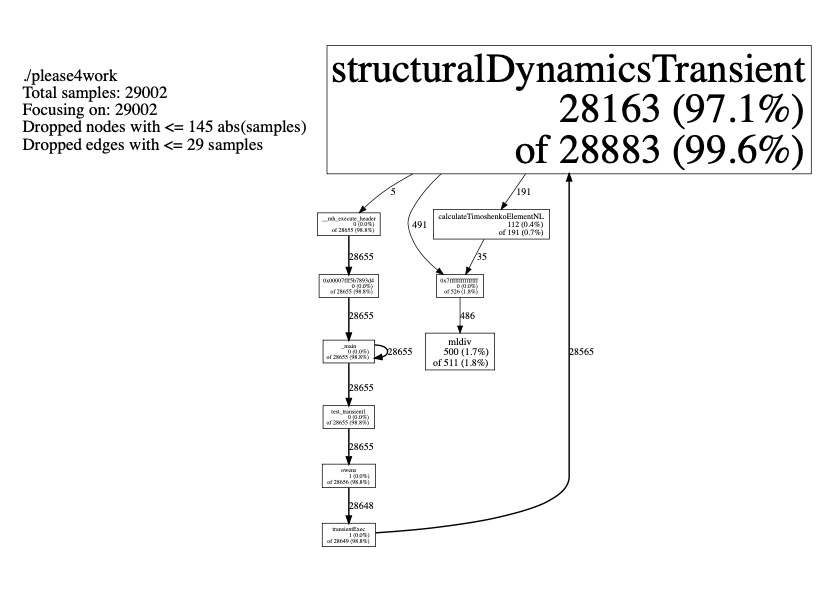
\includegraphics[width=0.99\textwidth]{../figs/profiler_output.png}
\vspace{-12pt}
\label{fig:ac_idx}
\end{figure}

\subsection{Debugging the Super Slow C++ Code}

So, it looks like there is some serious time being spent in the StructuralDynamicsTransient function, and not really the sub functions.  Looking at the code output, my best guess was that it was a memory issue where Matlab is very inefficiently forcing c++ to duplicate its memory management schemes, but as will be shown I was completely wrong.\\

After trying a few different debuggers/profilers to try to nail down exactly where the problem was, I switched to gdb. Some non-trivial issues getting it to run - keychain permissions, etc. Turns out none of them work on mac and you just have to run it as sudo.  The gdb debugger is terminal based and is invoked via the terminal from a folder that contains the source and working executable/binary.  The correct hooks have to be specified in the binary to get it to work together, and the debugger with binary has to be run in the same folder as the source code:

\begin{verbatim}
c++ -std=c++11 -g *.cpp -o nameofbinary
sudo gdb ./nameofbinary
\end{verbatim}

Using the gdb and the simple debugging principle that if the is one bottle neck taking a large amount of time, then there is a high probability randomly debugging and stopping the debugging will land you at the trouble spot.  Doing the process several dozen times yielded the following, all in structuralDynamicsTransient.cpp (keep in mind, it could have landed anywhere in the program).  By the way, this whole process of debugging Matlab C++ output is arduous: Change matlab code - Generate c++ code (~3min) - setup folder structure (30s) - compile c++ (30s) - get debugger running (2min) - step to desired location and print (1min). That's 7 minutes of overhead for each code change!

\begin{center}
\begin{tabular}{|c c|}
\hline
C++ Line & \# Hits \\
\hline
473 & 15 \\
\hline
429 & 5 \\
\hline
428 & 3 \\
\hline
471 & 1 \\
\hline
427 & 1 \\
\hline
472 & 1 \\
\hline

\end{tabular}
\end{center}

(\href{https://darkdust.net/files/GDB\%20Cheat\%20Sheet.pdf}{GDB Cheat Sheet}. Also, GDP print-outs of matrices are row major, even though they look column major, with gdb using the Matlab comma delimiter which makes it further look like it is row major when it is not. I lost a day of work because of this, so don't make the same mistake!) \\

They all map to a single Matlab line for basic matrix multiplication of fixed size matrices:
structuralDynamicsTransient.m:339

\begin{verbatim}
Kg = transMatrix'Kg*transMatrix;
\end{verbatim}

\noindent Why on earth it spits out the following nasty c++ code is a mystery yet to be solved, however, we can try to multiply the matrices in a different way.

\begin{verbatim}
  i = a->size[0] * a->size[1];
  a->size[0] = model_jointTransform->size[1];
  a->size[1] = model_jointTransform->size[0];
  emxEnsureCapacity_real_T(a, i);
  loop_ub = model_jointTransform->size[0];
  for (i = 0; i < loop_ub; i++) {
    m = model_jointTransform->size[1];
    for (boffset = 0; boffset < m; boffset++) {
      a->data[boffset + a->size[0] * i] = model_jointTransform->data[i +
        model_jointTransform->size[0] * boffset];
    }
  }

  if ((a->size[1] == 1) || (Kg->size[0] == 1)) {
    i = y->size[0] * y->size[1];
    y->size[0] = a->size[0];
    y->size[1] = Kg->size[1];
    emxEnsureCapacity_real_T(y, i);
    loop_ub = a->size[0];
    for (i = 0; i < loop_ub; i++) {
      m = Kg->size[1];
      for (boffset = 0; boffset < m; boffset++) {
        y->data[i + y->size[0] * boffset] = 0.0;
        inner = a->size[1];
        for (coffset = 0; coffset < inner; coffset++) {
          y->data[i + y->size[0] * boffset] += a->data[i + a->size[0] * coffset]
            * Kg->data[coffset + Kg->size[0] * boffset];
        }
      }
    }
  } else {
    m = a->size[0];
    inner = a->size[1];
    loop_ub = Kg->size[1];
    i = y->size[0] * y->size[1];
    y->size[0] = a->size[0];
    y->size[1] = Kg->size[1];
    emxEnsureCapacity_real_T(y, i);
    for (j = 0; j < loop_ub; j++) {
      coffset = j * m;
      boffset = j * inner;
      for (b_i = 0; b_i < m; b_i++) {
        y->data[coffset + b_i] = 0.0;
      }

      for (k = 0; k < inner; k++) {
        aoffset = k * m;
        totalNumDOF = Kg->data[boffset + k];
        for (b_i = 0; b_i < m; b_i++) {
          i = coffset + b_i;
          y->data[i] += totalNumDOF * a->data[aoffset + b_i];
        }
      }
    }
  }

  if ((y->size[1] == 1) || (model_jointTransform->size[0] == 1)) {
    i = Kg->size[0] * Kg->size[1];
    Kg->size[0] = y->size[0];
    Kg->size[1] = model_jointTransform->size[1];
    emxEnsureCapacity_real_T(Kg, i);
    loop_ub = y->size[0];
    for (i = 0; i < loop_ub; i++) {
      m = model_jointTransform->size[1];
      for (boffset = 0; boffset < m; boffset++) {
        Kg->data[i + Kg->size[0] * boffset] = 0.0;
        inner = y->size[1];
        for (coffset = 0; coffset < inner; coffset++) {
          Kg->data[i + Kg->size[0] * boffset] += y->data[i + y->size[0] *
            coffset] * model_jointTransform->data[coffset +
            model_jointTransform->size[0] * boffset];
        }
      }
    }
  } else {
    m = y->size[0];
    inner = y->size[1];
    loop_ub = model_jointTransform->size[1];
    i = Kg->size[0] * Kg->size[1];
    Kg->size[0] = y->size[0];
    Kg->size[1] = model_jointTransform->size[1];
    emxEnsureCapacity_real_T(Kg, i);
    for (j = 0; j < loop_ub; j++) {
      coffset = j * m;
      boffset = j * inner;
      for (b_i = 0; b_i < m; b_i++) {
        Kg->data[coffset + b_i] = 0.0;
      }

      for (k = 0; k < inner; k++) {
        aoffset = k * m;
        totalNumDOF = model_jointTransform->data[boffset + k];
        for (b_i = 0; b_i < m; b_i++) {
          i = coffset + b_i;
          Kg->data[i] += totalNumDOF * y->data[aoffset + b_i];
        }
      }
    }
  }
\end{verbatim}

\subsection{Matrix Multiplication Tweak}

\noindent By switching the multiplication to sparse matrices, you'd think it would output more complicated code, but it is just the opposite.  In Matlab this looks like:

\begin{verbatim}
Kg = full(sparse(transMatrix')*sparse(Kg)*sparse(transMatrix));
\end{verbatim}

\noindent  That one liner in Matlab was in its own function to start with, and now Matlab finally puts this in its own function in the C++ and the code is significantly simpler (and about a third the length), not to mention 24x faster.  Also, as a note, it didn't seem to have any effect when I tried to initialize variables outside of a for loop, it seemed to just do as it pleased, renaming variables and placing them wherever, etc.


\begin{center}
\begin{tabular}{|c| c c c c|}
\hline 
& Matlab & Matlab MEX & Compiled C++ & Octave \\
\hline
Execution Time Short (0.1s) \& File Output & 21s & NA & 5s & many minutes \\
\hline
Per 100 Steps & 7s & 2s & 5s & many minutes \\
\hline

\end{tabular}
\end{center}


\begin{verbatim}

static void applyConstraints(emxArray_real_T *Kg, const emxArray_real_T
  *transMatrix)
{
  emxArray_real_T *b_transMatrix;
  int i;
  int loop_ub;
  emxArray_real_T *this_d;
  int cend;
  emxArray_int32_T *this_colidx;
  int t3_m;
  emxArray_int32_T *this_rowidx;
  emxArray_real_T *t2_d;
  emxArray_int32_T *t2_colidx;
  emxArray_int32_T *t2_rowidx;
  emxArray_real_T *t3_d;
  emxArray_int32_T *t3_colidx;
  emxArray_int32_T *t3_rowidx;
  int this_m;
  int this_n;
  emxInit_real_T(&b_transMatrix, 2);
  i = b_transMatrix->size[0] * b_transMatrix->size[1];
  b_transMatrix->size[0] = transMatrix->size[1];
  b_transMatrix->size[1] = transMatrix->size[0];
  emxEnsureCapacity_real_T(b_transMatrix, i);
  loop_ub = transMatrix->size[0];
  for (i = 0; i < loop_ub; i++) {
    cend = transMatrix->size[1];
    for (t3_m = 0; t3_m < cend; t3_m++) {
      b_transMatrix->data[t3_m + b_transMatrix->size[0] * i] = transMatrix->
        data[i + transMatrix->size[0] * t3_m];
    }
  }

  emxInit_real_T(&this_d, 1);
  emxInit_int32_T(&this_colidx, 1);
  emxInit_int32_T(&this_rowidx, 1);
  emxInit_real_T(&t2_d, 1);
  emxInit_int32_T(&t2_colidx, 1);
  emxInit_int32_T(&t2_rowidx, 1);
  emxInit_real_T(&t3_d, 1);
  emxInit_int32_T(&t3_colidx, 1);
  emxInit_int32_T(&t3_rowidx, 1);
  b_sparse(b_transMatrix, t2_d, t2_colidx, t2_rowidx, &cend, &loop_ub);
  b_sparse(Kg, this_d, this_colidx, this_rowidx, &this_m, &this_n);
  d_sparse_mtimes(t2_d, t2_colidx, t2_rowidx, cend, this_d, this_colidx,
                  this_rowidx, this_n, t3_d, t3_colidx, t3_rowidx, &t3_m,
                  &loop_ub);
  b_sparse(transMatrix, t2_d, t2_colidx, t2_rowidx, &cend, &loop_ub);
  d_sparse_mtimes(t3_d, t3_colidx, t3_rowidx, t3_m, t2_d, t2_colidx, t2_rowidx,
                  loop_ub, this_d, this_colidx, this_rowidx, &this_m, &this_n);
  i = Kg->size[0] * Kg->size[1];
  Kg->size[0] = this_m;
  Kg->size[1] = this_n;
  emxEnsureCapacity_real_T(Kg, i);
  emxFree_real_T(&b_transMatrix);
  emxFree_int32_T(&t3_rowidx);
  emxFree_int32_T(&t3_colidx);
  emxFree_real_T(&t3_d);
  emxFree_int32_T(&t2_rowidx);
  emxFree_int32_T(&t2_colidx);
  emxFree_real_T(&t2_d);
  for (i = 0; i < this_n; i++) {
    for (t3_m = 0; t3_m < this_m; t3_m++) {
      Kg->data[t3_m + Kg->size[0] * i] = 0.0;
    }
  }

  for (loop_ub = 0; loop_ub < this_n; loop_ub++) {
    cend = this_colidx->data[loop_ub + 1] - 1;
    i = this_colidx->data[loop_ub];
    for (t3_m = i; t3_m <= cend; t3_m++) {
      Kg->data[(this_rowidx->data[t3_m - 1] + Kg->size[0] * loop_ub) - 1] =
        this_d->data[t3_m - 1];
    }
  }

  emxFree_int32_T(&this_rowidx);
  emxFree_int32_T(&this_colidx);
  emxFree_real_T(&this_d);
}
\end{verbatim}

\subsection{Other Types of Analyses}

When working on a different analysis portion (modal analysis), I had a similar speed issue where Matlab would run it in about 10 seconds, but the compiled C++ in about 60 seconds.  I followed the same debugging procedure and pinned it down to the Matlab built-in eig function.  I tried using different eig functions, different ways of formulating the input matrices, but there was no magic and the eig.cpp code is not pretty.  Also, a part of the structural code is a reduced order modal analysis, where only a subset of modes are calculated for speed.  However, Matlab does not support the required eigs function.  All of these performance issues are rooted in the base Matlab functions, which while they have been optimized for the Matlab runtime, don't seem to be as robust in c/c++ out of the box, but we will see how it can be made faster in the next section.


\section{Let Matlab Run the Compiler}

After all this, I installed Xcode as part of some Matlab-fortran experiments and in the process the C++ compilers were successfully linked to the Matlab Coder utility (had to install a specific old Xcode version not on the app store but rather via the official apple dev site \href{https://developer.apple.com/download/}{located here} that was compatible with my OS).  Letting Matlab run the compiler gave some impressive results with a 3x speedup compared to what it was before for the transient analysis per 100 timesteps, and a 5x speedup on the modal, but sadly still dismally slow (10min vs 80sec) for the flutter. While I did not try to profile the flutter analysis, the main difference between it and the modal analysis is that it wraps the modal analysis in fminbnd, a Matlab function.  It may be possible that the issue is somehow in the simple adjacent wrapper and it could be sped up by going through the process outlined above, but we may run into a dead end as well.  Here is the table on the transient analysis updated with the Matlab-driven compiled results:

\begin{center}
\begin{tabular}{|c| c c c c c|}
\hline 
& Matlab & MEX & Simply Compiled C++ & Matlab Compiled C++ & Octave \\
\hline
Short Exec (0.1s) \& File Output & 21s & NA & 5s & 2s & many minutes \\
\hline
Per 100 Steps & 7s & 2s & 5s & 1.5s & many minutes \\
\hline
\end{tabular}
\end{center}

Here is the output of what Matlab does to compiling a single file out of the 100 cpp files for the program.  As a note, it does take about 5-10 minutes to complete the compilation process...

\begin{lstlisting}
xcrun clang++ -c -isysroot /Applications/Xcode.app/Contents/Developer/Platforms/MacOSX.platform/Developer/SDKs/MacOSX10.13.sdk -arch x86_64 -std=c++11 -fno-common -fexceptions -mmacosx-version-min=10.9 -O3 -DMODEL=test_owens -DHAVESTDIO -DUSE_RTMODEL -DUNIX -I/Users/kevmoor/Documents/OWENS/src/codegen/exe/test_owens -I/Users/kevmoor/Documents/OWENS/src -I/Users/kevmoor/Documents/OWENS/src/codegen/exe/test_owens/examples -I/Applications/MATLAB_R2019b.app/extern/include -I/Applications/MATLAB_R2019b.app/simulink/include -I/Applications/MATLAB_R2019b.app/rtw/c/src -I/Applications/MATLAB_R2019b.app/rtw/c/src/ext_mode/common -I/Applications/MATLAB_R2019b.app/rtw/c/ert -o "fwrite.o" "/Users/kevmoor/Documents/OWENS/src/codegen/exe/test_owens/fwrite.cpp"
\end{lstlisting}

Then here is the command to link them all:

\begin{lstlisting}
xcrun clang++ -arch x86_64 -isysroot /Applications/Xcode.app/Contents/Developer/Platforms/MacOSX.platform/Developer/SDKs/MacOSX10.13.sdk -Wl,-rpath,/Applications/MATLAB_R2019b.app/bin/maci64 -Wl,-rpath,@executable_path -Wl,-rpath,@executable_path/. -L"/Applications/MATLAB_R2019b.app/bin/maci64" -o /Users/kevmoor/Documents/OWENS/src/test_owens rt_nonfinite.o rtGetNaN.o rtGetInf.o test_owens_rtwutil.o test_owens_data.o test_owens_initialize.o test_owens_terminate.o test_owens.o strcmp.o tic.o timeKeeper.o fileManager.o repmat.o find.o owens.o myfgetl.o fread.o feof.o sprintf.o str2double.o str2double1.o getSplitLine.o readMesh.o readBladeData.o importCactusFile.o readBCdata.o sort.o sortIdx.o readElementData.o readJointData.o readNodalTerms.o readInitCond.o readGeneratorProps.o createJointTransform.o calculateLambda.o eye.o xgetrf.o norm.o mtimes.o calculateBCMap.o readNLParamsFile.o transientExec.o processAeroLoadsBLE.o mapCactusLoadsFile.o readCactusGeom.o linear_interp.o sqrt.o calculateLoadVecFromDistForce.o calculateShapeFunctions.o sparse.o sparse1.o mtimes1.o fillIn.o initialElementCalculations.o ConcMassAssociatedWithElement.o calculateTimoshenkoElementInitialRun.o mldivide.o externalForcing.o structuralDynamicsTransient.o calculateTimoshenkoElementNL.o calculateTheo.o introsort.o insertionsort.o heapsort.o assembly.o applyBC.o qrsolve.o xgeqp3.o xzlarfg.o xzlarf.o xnrm2.o xgerc.o calculateReactionForceAtNode.o findElementsAssociatedWithNodeNumber.o elementPostProcess.o calculateStrainForElements.o fwrite.o modalExec.o staticAnalysis.o toc.o linearAnalysisModal.o assemblyMatrixOnly.o applyBCModal.o eigSolve.o schur.o xdhseqr.o xdlanv2.o xzggev.o xzggbal.o xzlartg.o xzhgeqz.o xztgevc.o extractFreqDamp.o writeOutput.o modalExecAuto.o fminbnd.o main.o test_owens_emxutil.o  -lm -lstdc++
\end{lstlisting}

\begin{figure}[htbp!]
\centering
%\vspace{-12pt}
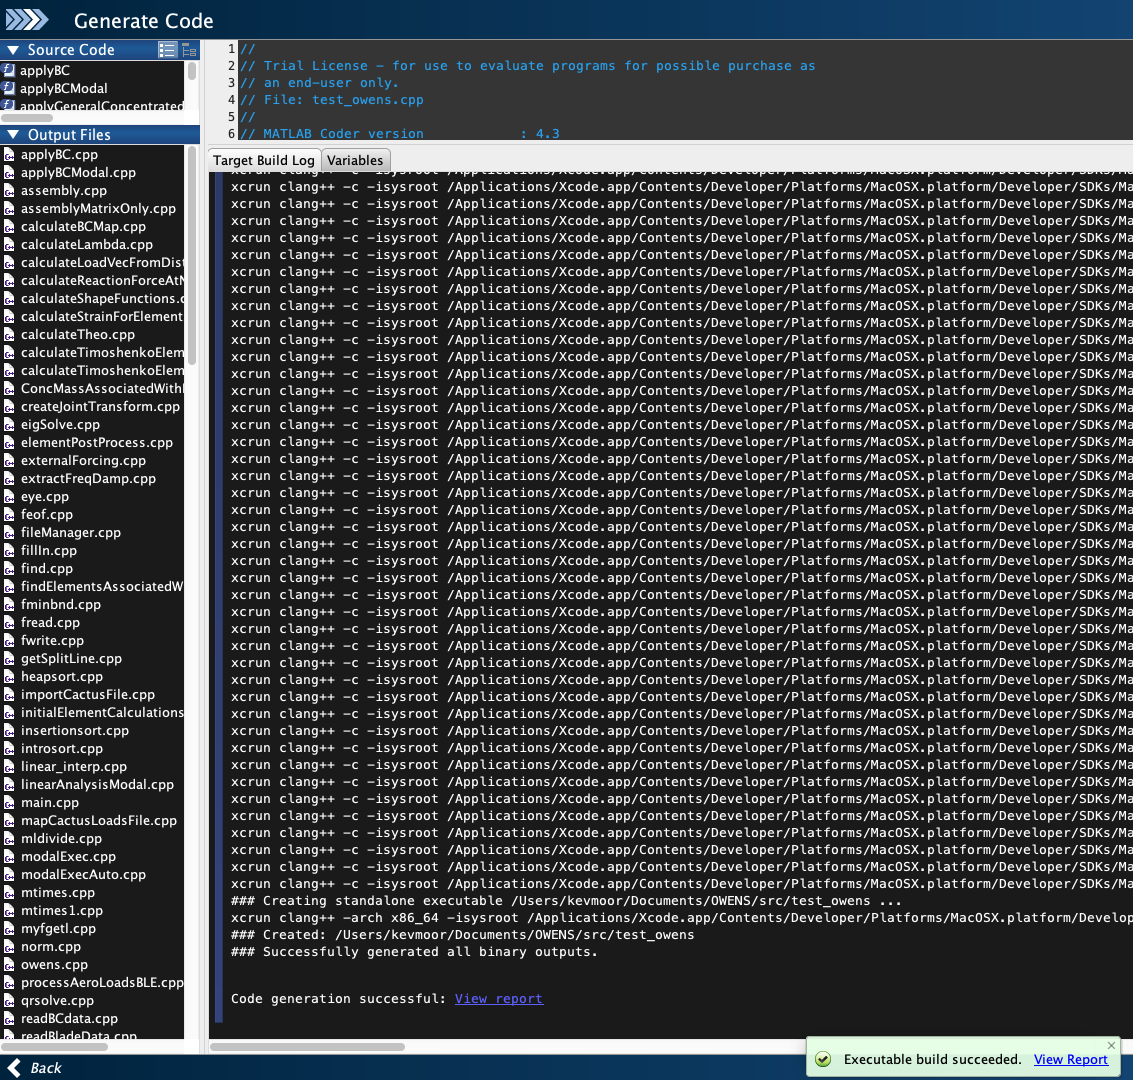
\includegraphics[trim={0 0 0 0},clip,width=0.99\textwidth]{../figs/compiler_output.png}
%\vspace{-12pt}
\caption{Coder output during compilation.}
\label{fig:compiler_output}
\end{figure}

\section{Summary}

Is it possible for Matlab to output fast C++ code? Yes and No, was about 5x faster than native Matlab (2019b) for the transient and modal analyses after all the tweaks, but about 7.5x slower for the flutter analysis (though I didn't go through the full profiling/debugging process for flutter).  Is the process to get there straightforward? No, requires about half the effort as porting to a different high-level language.  Is the output code unwieldy? Yes; I am not a CS major and wouldn't want to do anything more than just run it.  For this project: If I had to start over would I refuse to go the C++ automatic translation route? No, but I would point out the risks shown in this document.  Would I personally opt instead to put the effort into porting to a language like Julia? Yes.  Would I choose to write my own C++ code over letting Matlab do it? No, not for large codes. Would I choose to translate to Fortran code over the Matlab auto C++ translation process? Possibly, but not likely.\\

So, in summary, the Matlab to C/C++ automatic translation function is a feasible way to produce relatively well performing C/C++ code, though not without risk or potentially negative results depending on the desired application.

%I do recognize Matlab's value as a foolproof starter language and having good GUI capability, particularly for Simulink.  However, its greatest strength is also its worst weakness since it enables engineers to produce terrible code that works arguably well, enforcing bad habits that cost many times more than the multitude of Matlab licenses required for basic computation.  Consistent with its greatest strength/weakness, Matlab can be made to produce arguably well-performing C/C++ code, however the output code itself leaves much to be desired.\\

%If I could convince the reader to do so, I would recommend they consider the Julia language as it keeps the high level ease and simplicity of Matlab for syntax, while being in the same performance category as C, not to mention over 4000 open source mature libraries, an open source license, a Matlab comparable debugger, and all of the standard capabilities of a scientific computing based language (which for Matlab are quite limited when using Matlab as the master code and outputting C/C++).

\end{document}
